
% This LaTeX was auto-generated from MATLAB code.
% To make changes, update the MATLAB code and republish this document.

\documentclass{article}
\usepackage{graphicx}
\usepackage{color}

\sloppy
\definecolor{lightgray}{gray}{0.5}
\setlength{\parindent}{0pt}

\begin{document}

    
    \begin{verbatim}
c.g = 9.81; % ms/s^2
c.m = 0.142; % kg
c.L = .5; % m

options = odeset('Events', @event);

syms m g L theta thetadot thetaddot T

eqn(1) = m*(L*thetadot^2) == T - m*g*cos(theta);

eqn(2) = (thetaddot) == (-m*g*sin(theta))/(m*L);

x = solve(eqn,[T,thetaddot]);

syms theta(t) thetadot(t)
thetaEOM = subs(x.thetaddot,{'theta','thetadot'},...
               {theta,thetadot});
eom = odeFunction([thetadot;thetaEOM],[theta;thetadot],g,L);

hold on;

nat_freq = zeros(1,6);
releaseAngle = [5,10,15,30,60,90];
for i = 1:6
    j = releaseAngle(i);
    [Time,S,TE,SE,IE] = ode45(@(t,s)eom(t,s,c.g,c.L),linspace(0,10,1001),[(j*pi/180),0],options);
    plot(Time,S(:,1),'DisplayName', ['\theta_o = ' num2str(j) '^o']);
    xlabel('Time, sec');
    ylabel('\theta, rad');
    nat_freq(i) = 2*pi / (TE(2))
end
title('\theta vs Time');
legend('show')

figure(2)
hold on
plot(releaseAngle*pi/180,nat_freq, 'DisplayName', 'Measured Natural Frequency')
line([0  90].*pi/180, [sqrt(c.g/c.L),sqrt(c.g/c.L)],'Color','red','LineStyle','--',...
    'DisplayName',['Small Angle Approximation Natural Frequency'])
xlabel('\theta_o, rad');
ylabel('\omega_n, rad/s');
xticks([5*pi/180 pi/18 pi/12 pi/6 pi/3 pi/2])
xticklabels({'5\pi/180','\pi/18','\pi/12','\pi/6','\pi/3','\pi/2'})
xtickangle(45)
grid on
legend('show')
title('Natural Frequency (\omega_n) vs Inital Angle of Release (\theta_o)');

% set(gcf, 'PaperPositionMode', 'manual');
% set(gcf, 'PaperUnits', 'inches');
% set(gcf, 'PaperPosition', [1 1 6 2]);
% fig = gcf;
% print('BestFitFigure','-dpdf');



function [value isterminal direction] = event(t,s)
    value = s(2);
    isterminal(1) = false;
    direction(1) = -1;
end
\end{verbatim}

        \color{lightgray} \begin{verbatim}
nat_freq =

    4.4278         0         0         0         0         0


nat_freq =

    4.4278    4.4215         0         0         0         0


nat_freq =

    4.4278    4.4215    4.4110         0         0         0


nat_freq =

    4.4278    4.4215    4.4110    4.3543         0         0


nat_freq =

    4.4278    4.4215    4.4110    4.3543    4.1292         0


nat_freq =

    4.4278    4.4215    4.4110    4.3543    4.1292    3.7578

\end{verbatim} \color{black}
    
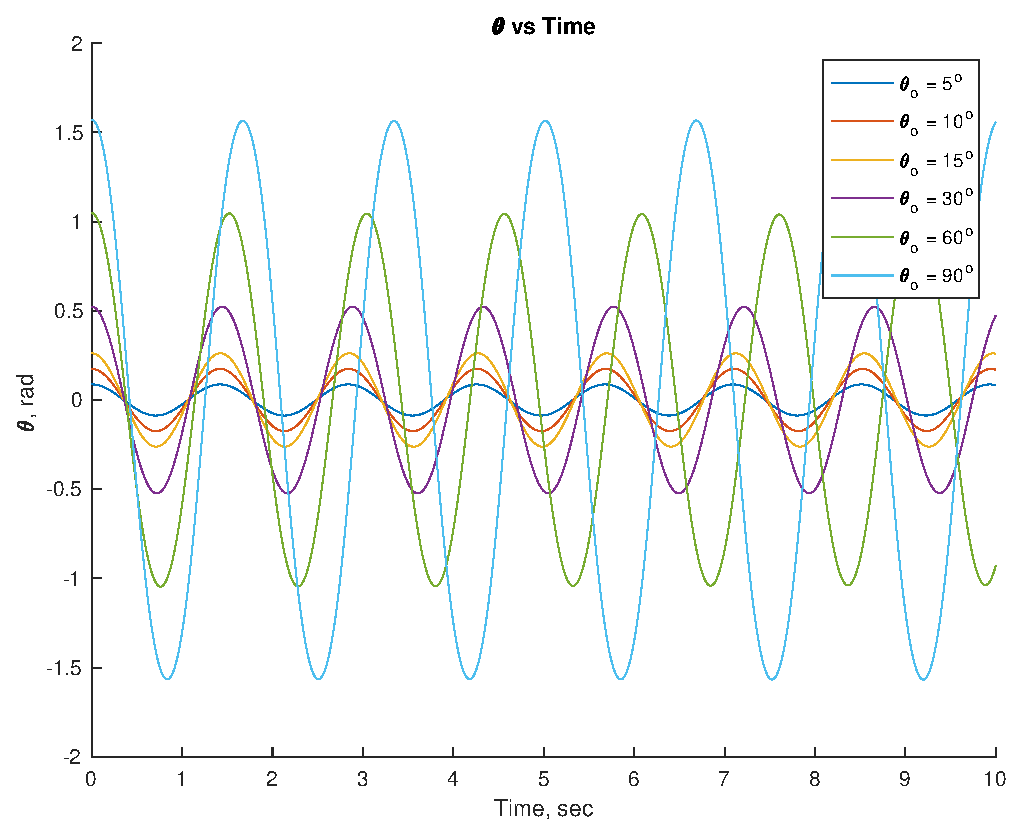
\includegraphics [width=4in]{Pendulum_01.eps}

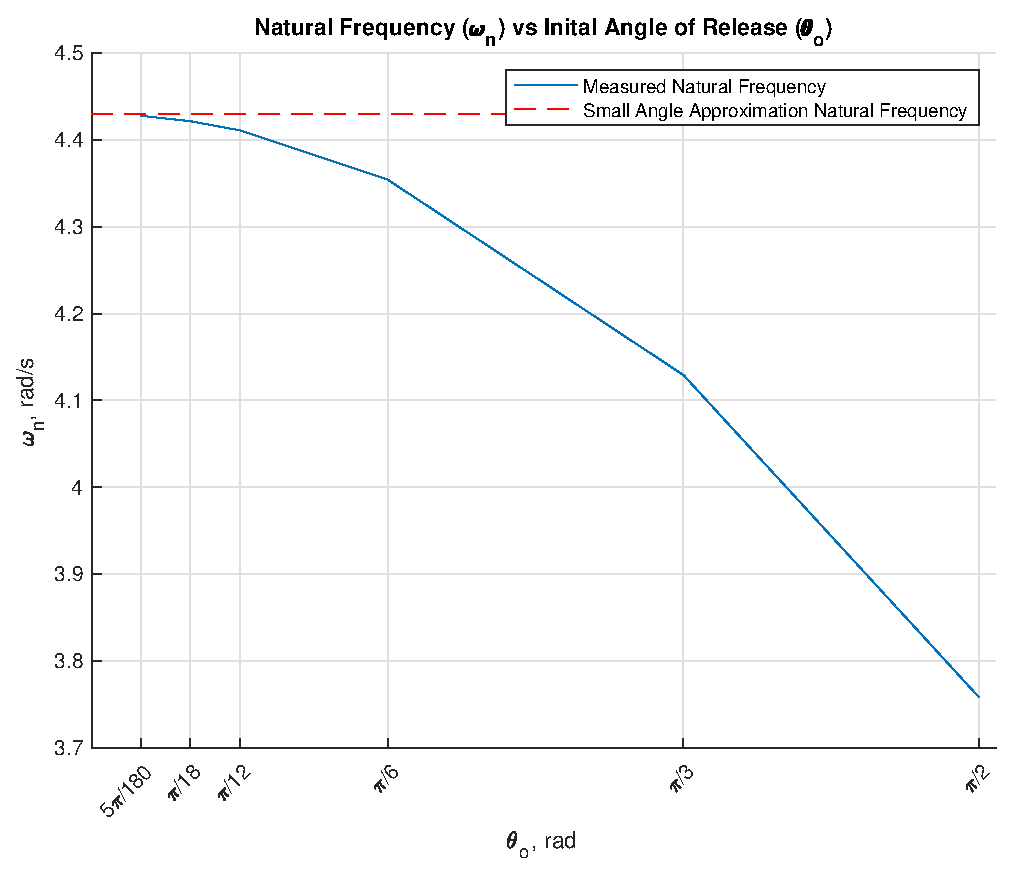
\includegraphics [width=4in]{Pendulum_02.eps}



\end{document}
    
